\documentclass[12pt,a4paper]{article}
\usepackage[a4paper,top=1.5cm, bottom=1.5cm, left=1.5cm, right=1.5cm]{geometry}
\usepackage[T2A]{fontenc}
\usepackage[utf8]{inputenc}
\usepackage[russian]{babel}
\usepackage{amsmath}
\usepackage{amssymb}
\usepackage{graphicx}
\usepackage{floatrow}
\usepackage{booktabs}
\usepackage{wrapfig}
\usepackage{indentfirst}
\usepackage{lipsum}
\usepackage{subcaption}
\usepackage{float}
\usepackage{enumitem}
\restylefloat{table}

\newcommand{\figref}[1]{(см. рис. \ref{#1})}
\newcommand{\e}[1]{\text{$\cdot10^{#1}$}}

\title{Лабораторная работа 5.4.2 \\ Исследование энергетического спектра $\beta$-частиц и определение их максимальной энергии при помощи магнитного спектрометра}
\author{Симанкович Александр\\ Б01-108}
\date{08.11.2023}

\begin{document}
	\maketitle
	
	\section*{Аннотация}
	
	В работе экспериментально исследуется энергетический спектр $\beta$-частиц $^{137}$Cs. В качестве экспериментальной установки используется магнитный спектрометр. Определяется максимальная энергия $\beta$-частиц при распаде  $T_{max} = (570 \pm 25)$ кэВ. Калибровка производится по положению конверсионного пика $T_k = 624$ кэВ.
	
%	В работе экспериментально подтвержден эффект электронного парамагнитного резонанса в молекуле дифенилпикрилгидразила (ДФПГ). Подтверждена теоретическая зависимость резонансной частоты от значения магнитного поля. Получен $g$-фактор несвязанного электрона в молекуле ДФПГ $g = (1.94 \pm 0.04)$ . Оценено время релаксации электрона в молекуле ДФПГ $\tau = (15.0 \pm 1.0)$ нс.
	
	\section*{Теоретическое введение}
	
	\subsection*{Основы $\beta$-распада}
	
	$\beta$-распад -- явление самопроизвольного превращения ядер, в котором массовое число $A$ ядра сохраняется, а заряд изменяется на единицу. Ядра, подверженные $\beta$-распаду встречаются во всей области значений массового числа $A$. Диапазон энергий, высвобождаемых при $\beta$-распаде: $18 \text{ кэВ} \div 13.4 \text{ МэВ}$. Периоды полураспада лежат в пределах $10^{-6} \text{ с} \div 10^{18} \text{ лет}$.
	
	В данной работе изучается бета-минус-распад ($\beta^{-}$) ядра $^{137}$Cs:
	
	\begin{equation}
		^A_Z X \rightarrow ^{A}_{Z+1} X + e^{-} + \tilde{\nu}.
	\end{equation}
	В данном типе распада испускается электрон и антинейтрино.
	
	Поскольку масса ядра много больше массы электрона $A \cdot m_{p} \gg m_{e}$, энергия, уносимая ядром, очень мала. Однако, в эксперименте у электронов наблюдается сплошной спектр, который объясняется существованием антинейтрино, которое в состоянии унести оставшуюся энергию. Таким образом, электроны могут иметь любую энергию от нулевой до полной энергии, выделяемой при $\beta$-распаде $T_{max}$.
	
	\subsection*{Спектр $\beta$-электронов}
	
	Как было отмечено выше, спектр является непрерывным от нуля до $T_{max}$. $W$ -- спектральная плотность вероятности.
	
	Спектр $\beta$-электронов для разрешенных фермиевских переходов может быть рассчитан теоретически. В этом случае вероятность $\beta$-распада с заданными $p_e$ и $p_{\nu}$ пропорциональна статистическому весу. Поскольку энергия, уносимая ядром, мала, мы можем считать, что $T_e + E_{\nu} = T_{\beta} = T_{max}$. Тогда энергия и импульс нейтрино полностью определяются $p_e$.
	
	\begin{wrapfigure}[15]{r}{7.0cm}
		%              ^^ number of occupied rows
		\includegraphics[scale=0.6]{res/spectrum.png}
		\caption{Спектр $\beta$-электронов.}
		\label{fig:spectrum}
		\vspace{0pt}
	\end{wrapfigure}
	
	Интервалу $(p_e; p_e + d p_e)$ соответствует фазовый объем $4 \pi p_e^2$. Аналогичный шаровой слой соответствует антинейтрино: $4 \pi p_{\nu}^2$. Тогда получаем:
	\begin{equation}
		W(p_e) dp_e \propto p_e^2 p_{\nu}^2 dp_e.
		\label{eq:probability}
	\end{equation}
	
	Выразим импульс антинейтрино:
	\begin{equation}
		p_{\nu} = E_{\nu} / c = \frac{T_{max} - T_e}{c}.
		\label{eq:impulse_nu}
	\end{equation}
	
	Подставляя \eqref{eq:impulse_nu} в \eqref{eq:probability} получаем:
	\begin{equation}
		W(p_e) dp_e \propto p_e^2 (\sqrt{p_{max}^2 + m_e^2 c^2} - \sqrt{p_e^2 + m_e^2 c^2})^2 dp_e.
	\end{equation}
	
	На спектре \figref{fig:spectrum} также наблюдается выраженный пик при $p_e = p_{\text{конв}}$. Этот пик называется конверсионным. При $\beta$-распаде ядро может оказаться возбужденным. Энергия возбуждения может быть излучена через $\gamma$-квант или передана электрону с внутренней оболочки атома. Эти электроны образуют монохроматический пик. Для $^{137}$Cs он расположен на энергии $T_{\text{к}} = 0.624$ МэВ.
	
	\section*{Методика эксперимента}
	
	\begin{figure}[H]
		\centering
		\begin{minipage}{0.5\textwidth}
			\centering
			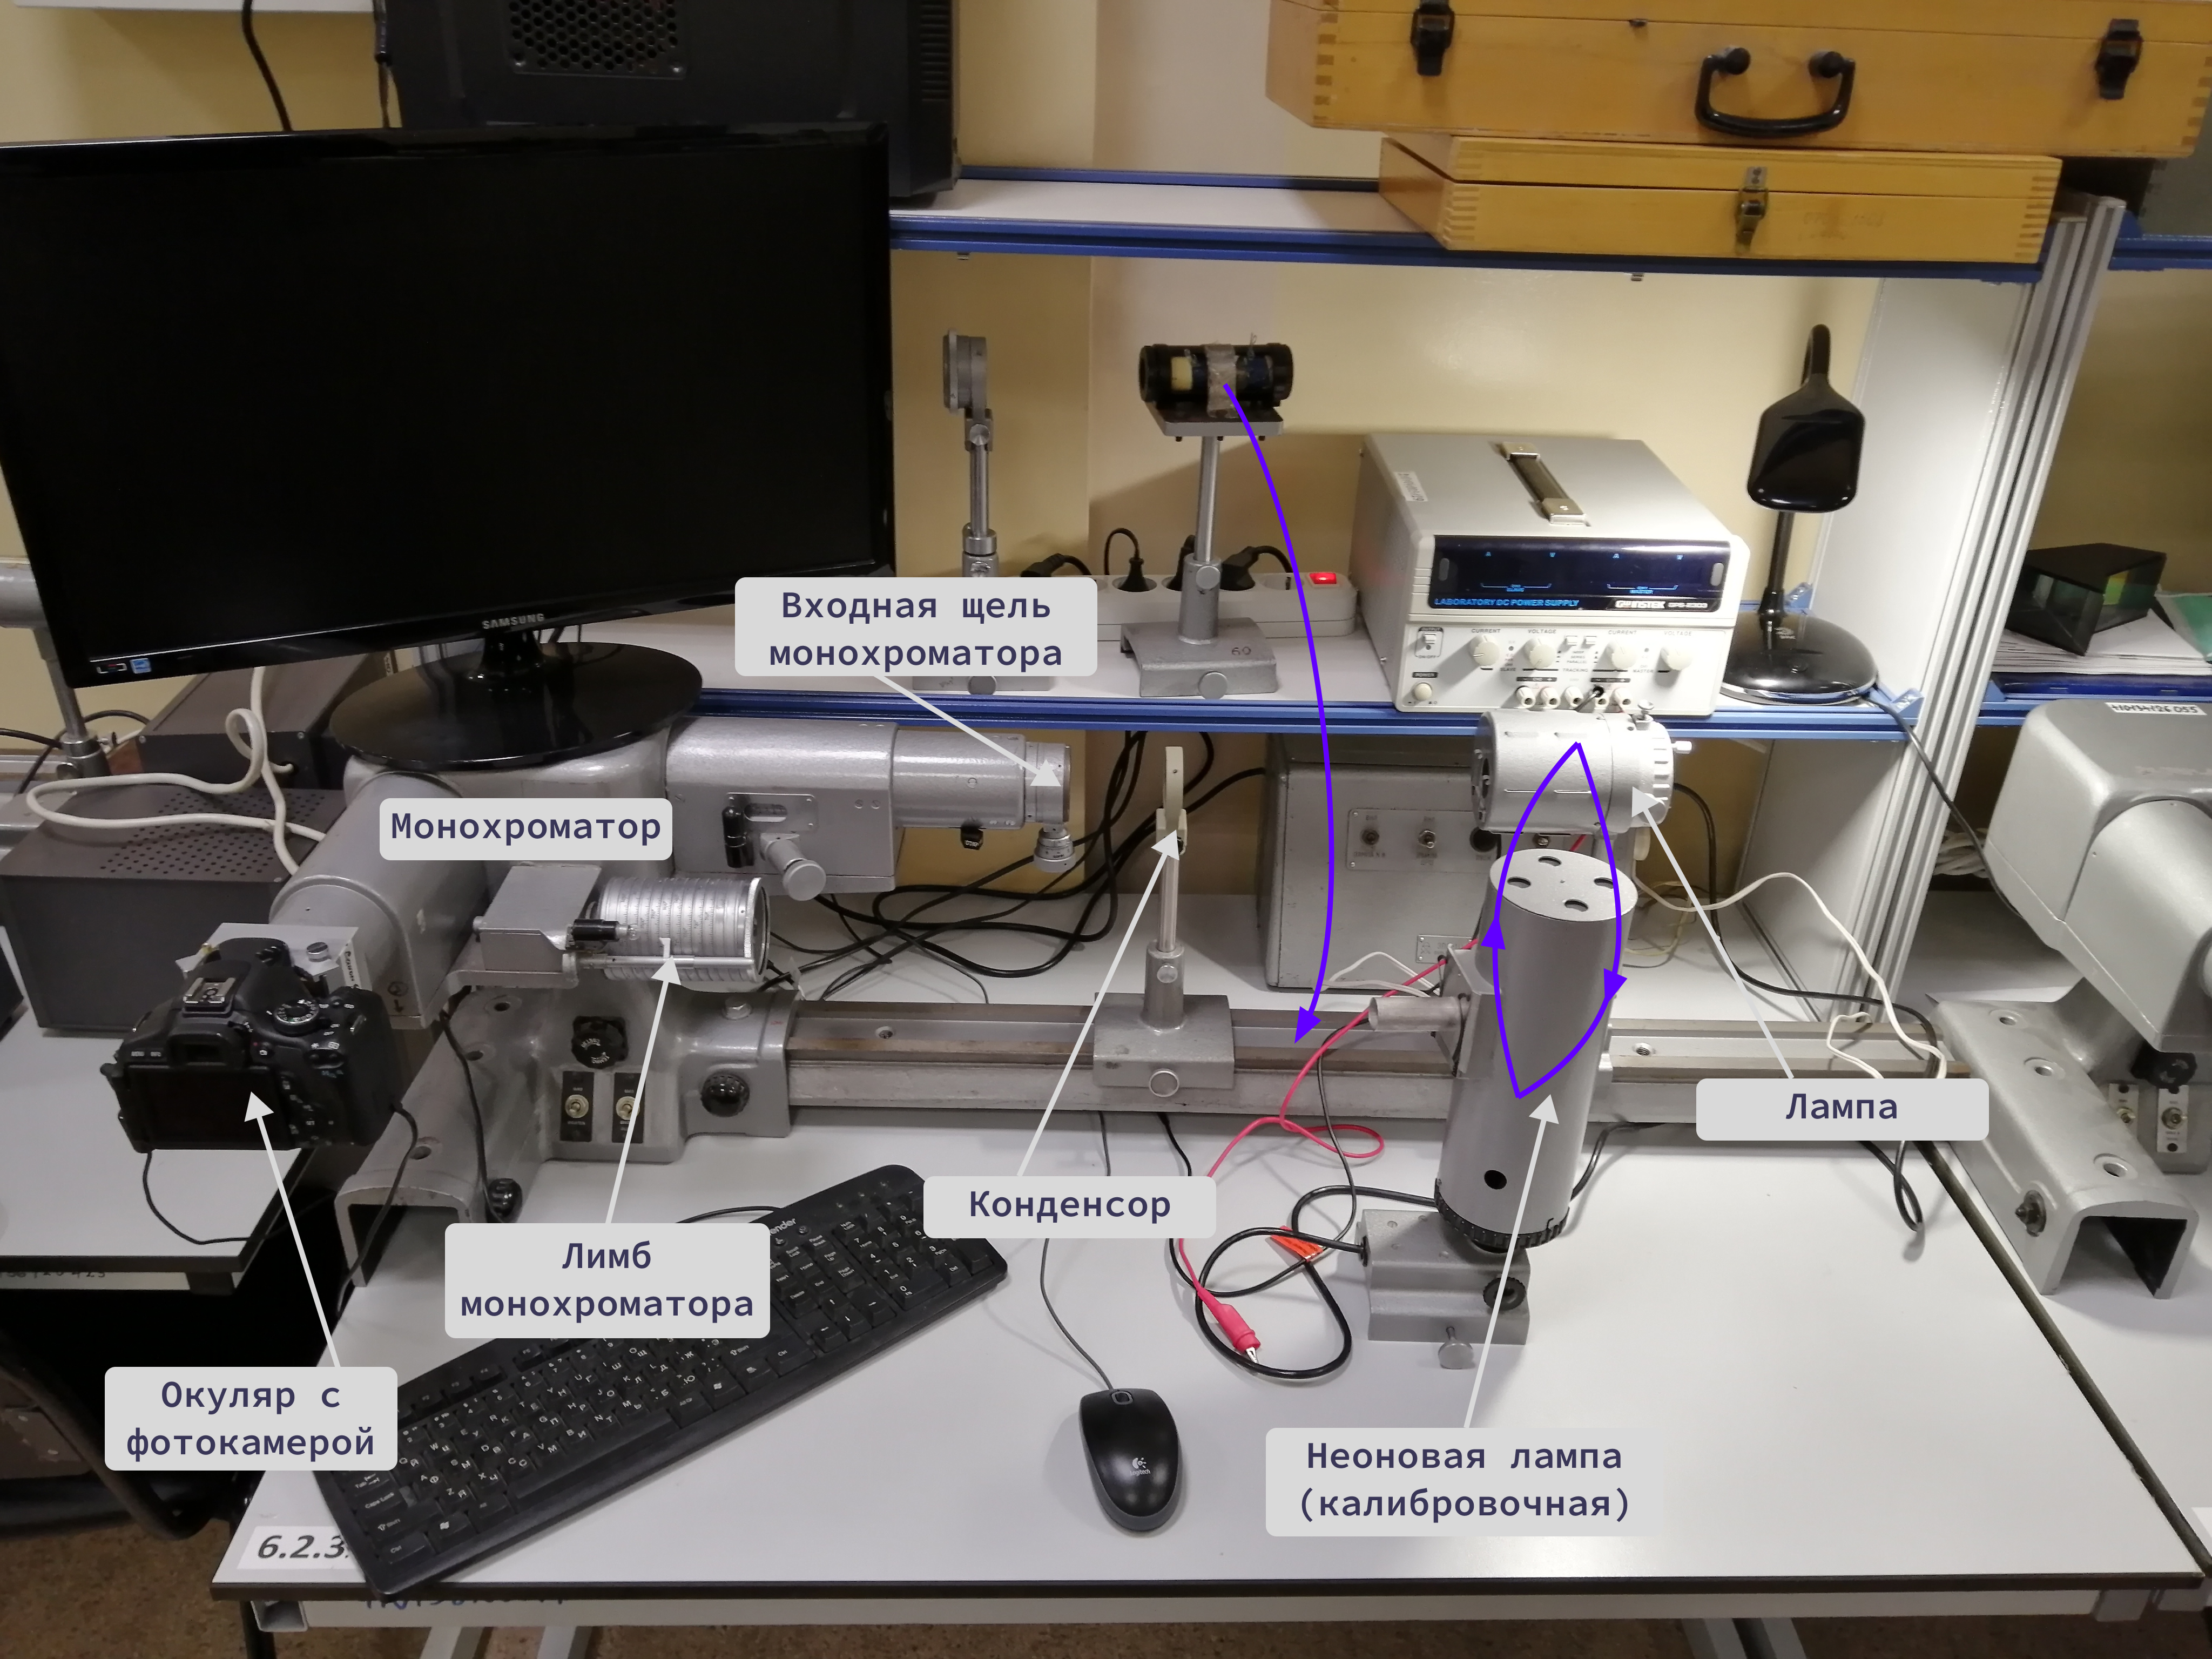
\includegraphics[width=1.0\linewidth]{res/setup.png}
		\end{minipage}%
		\begin{minipage}{0.5\textwidth}
			\centering
			\includegraphics[width=1.0\linewidth]{res/scheme.png}
		\end{minipage}
		\caption{Схема установки для изучения $\beta$-распада.}
		\label{fig:setup_scheme}
	\end{figure}
	
	\begin{figure}[H]
		\centering
		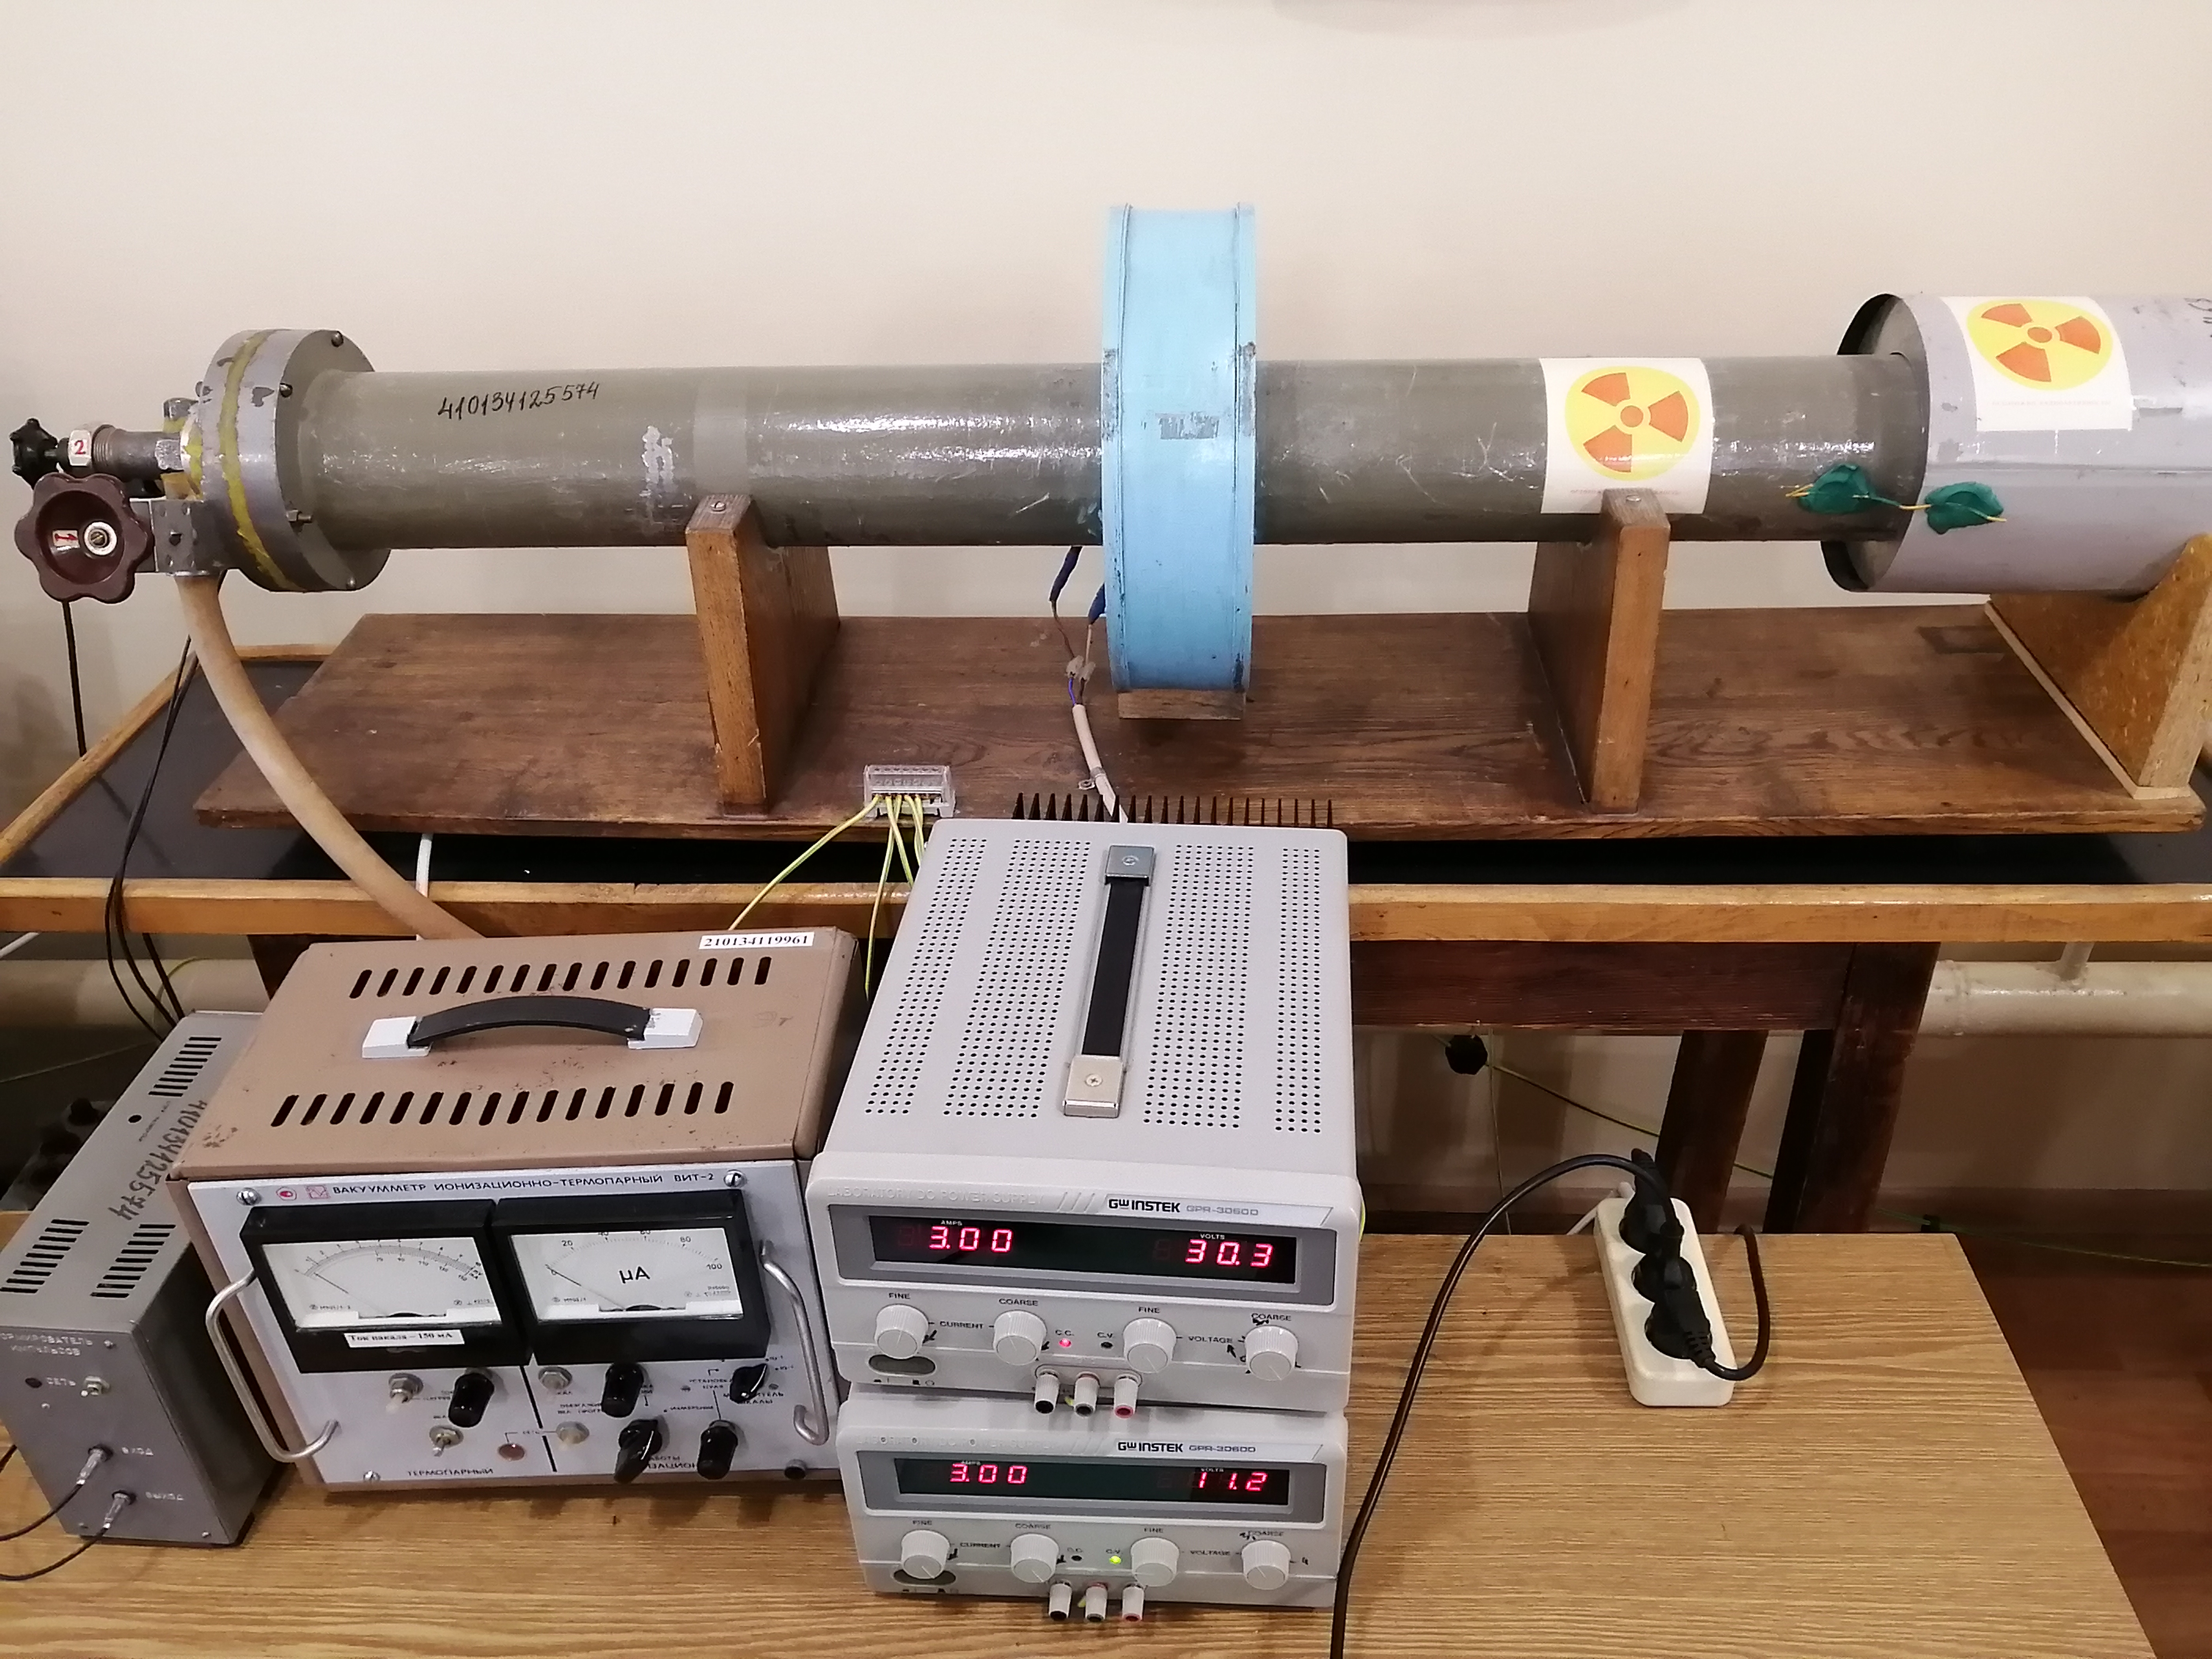
\includegraphics[width=0.6\linewidth]{photos/setup.jpg}
		\caption{Фото установки для изучения $\beta$-распада.}
		\label{fig:setup_photo}
	\end{figure}
	
	Для определения энергии $\beta$-частиц используется $\beta$-спектрометр с "короткой линзой" \; \figref{fig:setup_scheme}. Электроны, испускаемые источником, попадают в магнитное поле катушки (магнитной линзы). В фокусе этой линзы расположен счетчик -- сцинтиллятор. Сигнал с сцинтиллятора попадает в ФЭУ, после чего с помощью АЦП сохраняется на компьютере.
	
	Для предотвращения попадания прямого $\gamma$-излучения и $\beta$-частиц устанавливается свинцовый фильтр. Магнитная линза имеет значительные сферические аберрации, для исключения их влияния необходимо устанавливать диафрагму.
	
	Для исключения рассеяния электронов в спектрометре с помощью форвакуумного насоса поддерживается давление $P \sim 0.1$ Торр.
	
	Для фокусного расстояния линзы можно показать, что:
	\begin{equation}
		\frac{1}{f} \propto \frac{I^2}{p_e^2},
		\label{eq:focus}
	\end{equation}
	где $I$ -- сила тока в линзе. При заданной силе тока в счетчик попадают электроны с импульсом $p_e \pm \Delta p_e / 2$. $\Delta p_e$ -- разрешающая способность спектрометра.
	
	Геометрия прибора не изменяется в ходе опыта, поэтому
	\begin{equation}
		p_e = kI,
	\end{equation}
	где $k$ -- константа прибора.
	
	Рассмотрим связь частоты регистрации частиц и спектральной плотности вероятности.
	$$N(p_e) = W(p_e) \cdot \Delta p_e.$$
	
	Исходя из \eqref{eq:focus} получим:
	$$ \Delta p_e = \frac{1}{2} \frac{\Delta f}{f} 	p_e.$$
	
	Тогда:
	\begin{equation}
		N(p_e) = C \cdot W(p_e) p_e
		\label{eq:fermi}
	\end{equation}
	
	\section*{Результаты}
	
	Проведем измерения частоты регистрации частиц для токов в диапазоне $I = (0.0 \div 4.2)$ А. Каждое измерение проводится в течение 100 секунд. Для учета фона вычтем из $N$ значение $N_0$ при $I = 0$ А.
	
	\begin{figure}[H]
		\centering
		\includegraphics[width=0.9\linewidth]{gen/spectrum.pdf}
		\caption{Зависимость частоты регистрации частиц от тока.}
		\label{fig:exp_spectrum}
	\end{figure}

	На графике наблюдается конверсионный пик. Для $^{137}$Cs он расположен на $T_k = 624$ кэВ. Таким образом, нормируем график по энергии и импульсам $T_e$, $p_e$ \figref{fig:exp_spectrum}.
	
	Исходя из ширины конверсионного пика оценим разрешающую способность спектрометра.
	$$ \Delta p_e \approx 20 \text{ кэВ}/\mathcal{C}.$$
	
	
	\begin{table}[H]
		\footnotesize
		\input{gen/data.tex}
		\caption{Исходные и обработанные данные эксперимента.}
		\label{tab:data}
	\end{table}

	В соответствии с \eqref{eq:fermi} построим график Ферми.
	$$ \sqrt{N(p_e)} \cdot p_e^{-3/2} \propto T_{max} - T.$$

	\begin{figure}[H]
		\centering
		\includegraphics[width=0.9\linewidth]{gen/fermi.pdf}
		\caption{Зависимость частоты регистрации частиц от тока.}
		\label{fig:exp_fermi}
	\end{figure}
	
	На графике есть линейный участок, его экстраполяция пересекает ось абсцисс в точке $T = T_{max}$.
	
	\begin{table}[H]
		\footnotesize
		\input{gen/mnk.tex}
		\caption{Аппроксимация линейного участка.}
		\label{tab:mnk}
	\end{table}
	
	$$T_{max} = \frac{-b}{a} = (572 \pm 25) \text{ кэВ}.$$
	
	Построим теоретическую зависимость $N(I)$ исходя из \eqref{eq:probability}.
	
	\begin{figure}[H]
		\centering
		\includegraphics[width=0.9\linewidth]{gen/spectrum_fermi.pdf}
		\caption{Зависимость частоты регистрации частиц от тока.}
		\label{fig:th_spectrum}
	\end{figure}
	
	Как можно видеть, теоретическая зависимость хорошо описывает экспериментальный результат.
	
	\section*{Заключение и выводы}
	
	В работе определено значение максимальной энергии $\beta$-частиц при распаде $^{137}$Cs $T_{max} = (570 \pm 25)$ кэВ.
	
	Подтверждена теоретическая зависимость $N(p_e)$.
	
	Определено значение разрешающей способности спектрометра $\Delta p_e \approx 20 \text{ кэВ}/{\mathcal{C}}$.
\end{document}
